% DOC SETTINGS ===================================
\documentclass{article}
\usepackage[utf8]{inputenc}
\usepackage{steinmetz}
\usepackage{mathtools}  
\usepackage{multicol}
\usepackage{circuitikz}
\usepackage{tikz}
\usepackage{listings}
\usepackage{geometry}
\usepackage{fancyhdr}
\usepackage{graphicx}
\usepackage{minted} 
\usepackage[numbered,framed]{matlab-prettifier}
\usepackage{lmodern}
\usepackage{amsfonts}
\usepackage{media9}
\usepackage{parskip}
\definecolor{bg}{rgb}{0.95,0.95,0.95}
\usetikzlibrary{positioning, fit, calc}
\pagestyle{fancy}
\lhead{ECE2714 Project}
\rhead{Kavin Thirukonda 2021}
\usepackage{mdframed}
\surroundwithmdframed{minted}
\fancyheadoffset{0mm}
 \geometry{
 a4paper,
 total={170mm,257mm},
 left=20mm,
 top=25mm,
 }
\mathtoolsset{showonlyrefs} 
\cfoot{}
% DOC SETTINGS ===================================
\begin{document}
\section*{Part 1: Anti-Aliasing Filter}
\begin{enumerate}
    \item Using the Analog Filter Wizard, design a fourth-order (2-stage) Sallen-Key low-pass Butterworth filter (determine the values of resistors and capacitors in the circuit diagram above) to achieve the following performance characteristics:
    \begin{itemize}
        \item Pass-band: 0 dB gain at DC to -3 dB gain at 3.1 kHz
        \item Stop-band: $\leq$ -20 dB gain for frequencies above 6 kHz
    \end{itemize}
    \item Simulate your circuit designed above in LTSpice. You may use an ideal op-amp model or a realistic op-amp model. You should use standard resistor and capacitor values nearest to the values found in 1 (those that would be found in your lab-in-box kit). Perform the following analyses. We suggest making a separate file for each analysis. Copy the file and adjust the parameters.
    \begin{center}
            \boxed{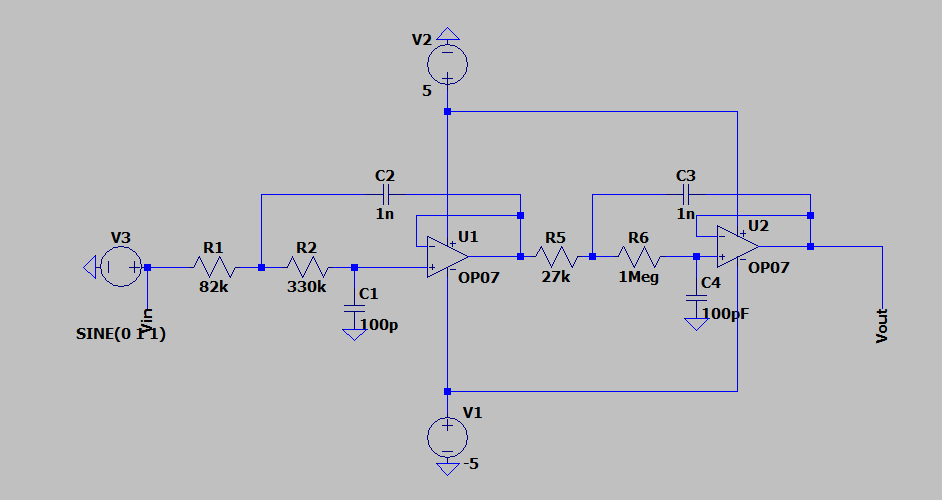
\includegraphics[width = .95\textwidth]{p1p2.png}}
    \end{center}
    \item Compute an expression for the theoretical frequency response of the filter using your standard component values from 2. In other words, find $H(j\omega)$
    \begin{center}
        First we calculate the values for the first stage of the filter
    \end{center}
    \begin{equation}
        H_1(j\omega): \alpha = \frac{R_1+R_2}{2R_1R_2C_1} = \frac{82k\Omega+330k\Omega}{2(82k\Omega)(330k\Omega)(1nF)} = 7612.71
    \end{equation}
    \begin{equation}
        H_1(j\omega): \omega_o^2 = \frac{1}{R_1R_2C_1C_2} = \frac{1}{(82k\Omega)(330k\Omega)(1nF)(100pF)} = 369549150
    \end{equation}
    \begin{center}
        Next we can calculate the values for the second stage
    \end{center}
    \begin{equation}
        H_2(j\omega): \alpha = \frac{R_1+R_2}{2R_1R_2C_1} = \frac{27k\Omega+1M\Omega}{2(27k\Omega)(1M\Omega)(1nF)} = 19018.52
    \end{equation}
    \begin{equation}
        H_2(j\omega): \omega_o^2 = \frac{1}{R_1R_2C_1C_2} = \frac{1}{(27k\Omega)(1M\Omega)(1nF)(100pF)} = 370370370.4
    \end{equation}
    \begin{center}
        Then we can multiply the frequency responses in time to get the overall frequency response of the system.
    \end{center}
    \begin{align}
        H(j\omega) &= H_1(j\omega) * H_2(j\omega)\\
        &= \frac{\omega_o^2}{\omega_o^2-\omega^2+j2\alpha\omega} \cdot \frac{\omega_o^2}{\omega_o^2-\omega^2+j2\alpha\omega}\\
        &= \boxed{\frac{369549150}{369549150-\omega^2+j2\cdot7612.71\omega} \cdot \frac{370370370.4}{370370370.4-\omega^2+j2\cdot19018.52\omega}}\\
    \end{align}
    \item Plot a Bode plot of the theoretical frequency response from 3 using Matlab or a similar tool. Overlay the points that correspond to the results of the simulation in 2.a by measuring the gain and phase shift from the input-output time plots. Be sure to convert to appropriate units (e.g., dB).
    \lstinputlisting[style=Matlab-editor]{s1p5.m}
    \begin{center}
        \boxed{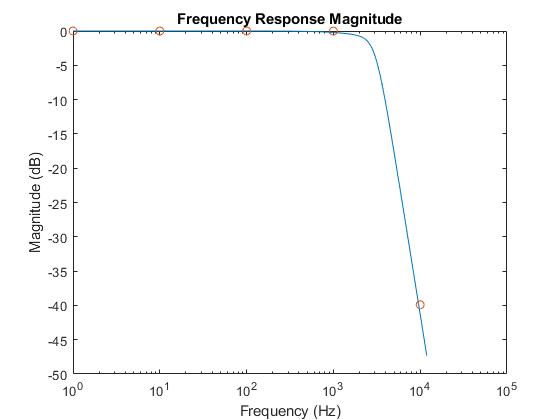
\includegraphics[width = .45\textwidth]{s1p5mag.png}}
        \boxed{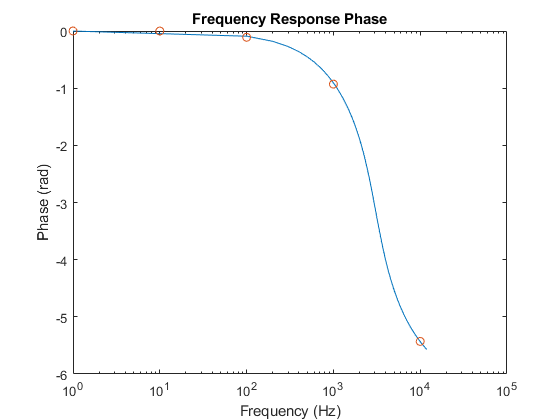
\includegraphics[width = .45\textwidth]{s1p5phase.png}}
    \end{center}
    \newpage
    \item Using the wav2spice tool (see below) and the linear approximation option, create a PWL file for use as a voltage source in LTSpice from the file corrupted.wav.
    \begin{center}
        \boxed{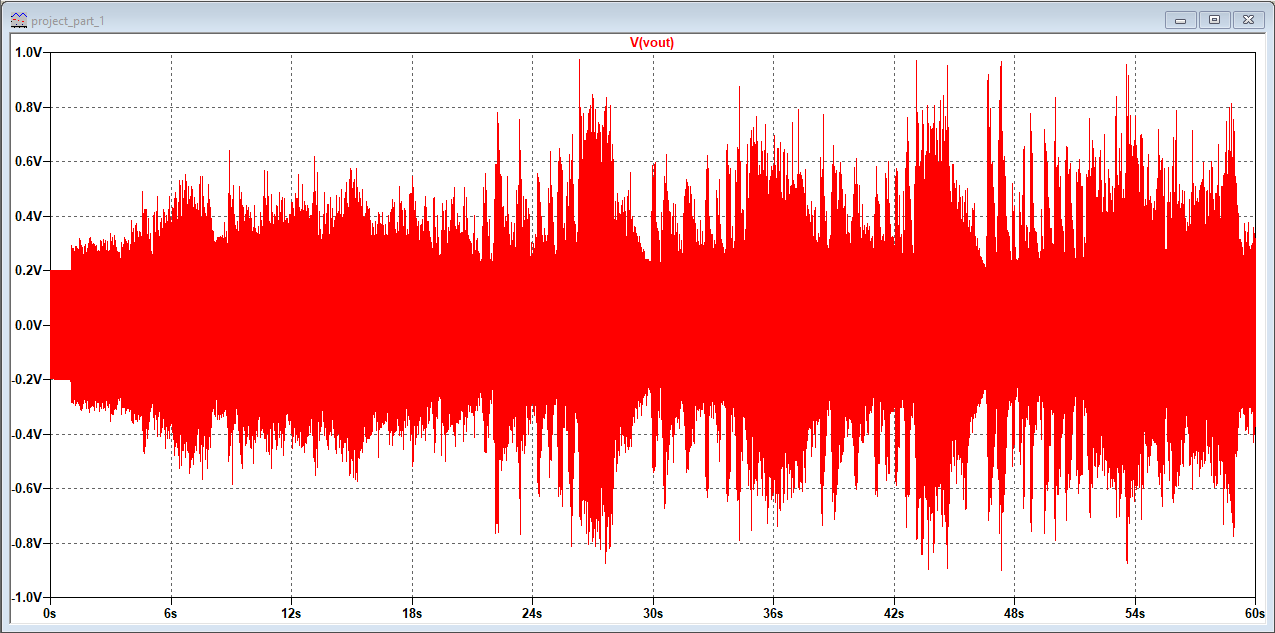
\includegraphics[width = .9\textwidth]{filtercorrupted.png}}
    \end{center}
    \item Repeat step 5 but using a simple voltage source and 1-ohm resistor as the circuit model. Save the resistor voltage to a different ASCII file, e.g. noaafilter-output.txt. Again, this may take several minutes.
    \begin{center}
        \boxed{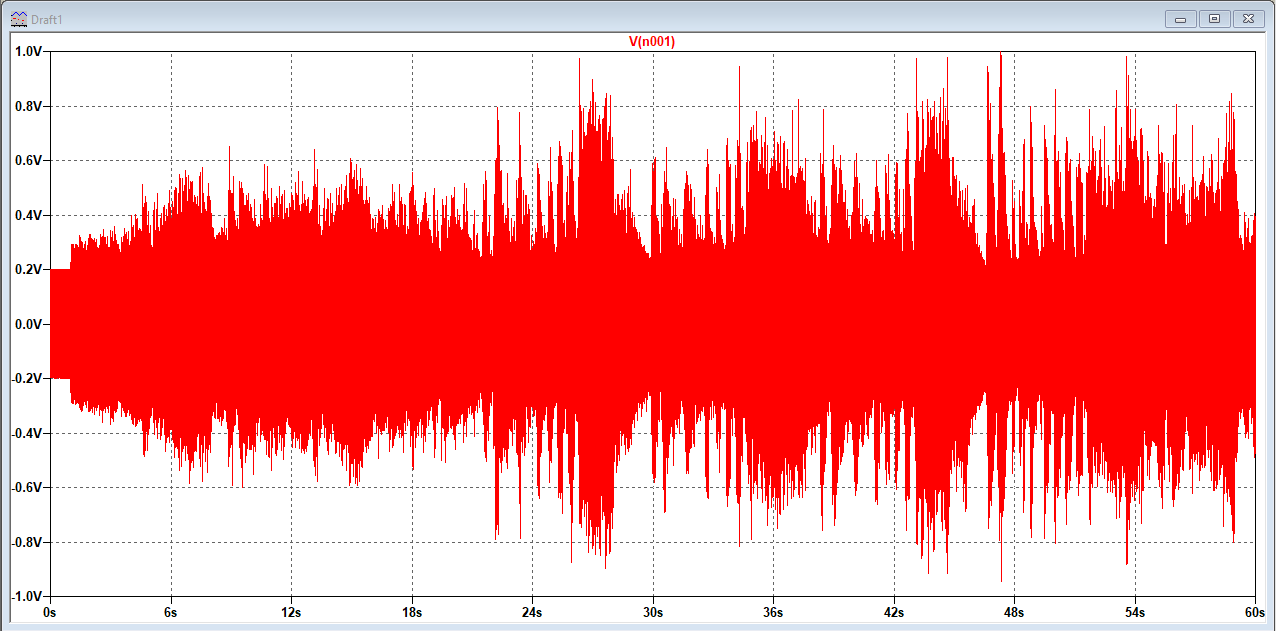
\includegraphics[width = .9\textwidth]{nofiltercorrupted.png}}
    \end{center}
    \item Using the spice2wav tool (see below), convert the files in steps 5 and 6 to wav files using a sampling rate of 6000 Hz. This simulates the ADC block.
    \item Document your completion of Part I in the project report:
    \begin{enumerate}
        \item Describe the purpose of Part I in your own words as it relates to the course content.
        \begin{center}
            Part one of this project give the student a good understanding of how filters are typically designed in practice, i.e. using the filter wizard, how they can be simulated, and tested using multiple programs. This lets us see the correlation between the formulas we are using and the simulation software LTSpice and give a bit of background on what LTSpice is doing when a circuit is being simulated.
        \end{center}
        \item List the component values that correspond to your design and the standard values chosen.
        \begin{center}
            Filter 1:
        \end{center}
        \begin{equation}
            R_1 = 82k\Omega, R_2 = 330k\Omega, C_1 = 1nF, C_2 = 100pF
        \end{equation}
        \begin{center}
            Filter 2:
        \end{center}
        \begin{equation}
            R_1 = 27k\Omega, R_2 = 1M\Omega, C_1 = 1nF, C_2 = 100pF
        \end{equation}
        \item Display a screenshot of your simulated circuit in step 2.
        \begin{center}
            The circuit can be seen above in the section for step 2.
        \end{center}
        \item Compare the behavior of your simulated circuit to that expected by your theoretical analysis by referring to the specific measurements made. Generate plots or tables as needed to support your comparison.
        \begin{center}
            As can be seen in the plots for question four, the theoretical values match the simulated almost exactly, on that plot the points are representations of the ltspice values for 1Hz, 10Hz, 100Hz, 1kHz, and 10kHz. For each of those point overlayed on the theoretical value it shows that it matches up on the various places for both phase and magnitude.
        \end{center}
        \item Describe your observations from step 7.
        \begin{center}
            It seems like the triangle gets removed, which makes sense because triangles seems like they emit a high frequency sound (i think?)
        \end{center}
    \end{enumerate}
\end{enumerate}
\newpage
\section*{Part 2: Digital Filtering}
\begin{enumerate}
    \item Use the Matlab tool iirnotch to design a second-order IIR notch filter to remove the corrupting signal.
    \lstinputlisting[style=Matlab-editor]{s2p1.m}
    \begin{center}
        \boxed{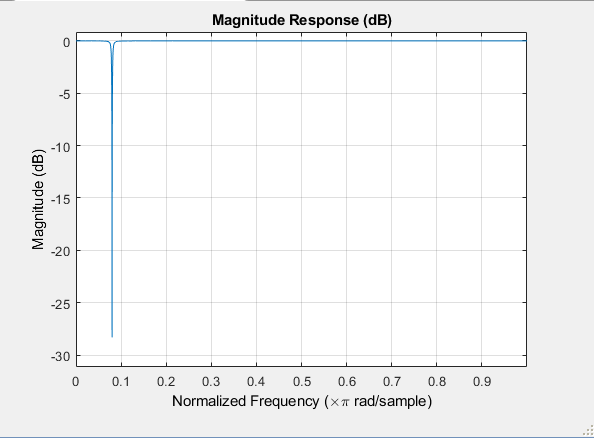
\includegraphics[width = .65\textwidth]{s2p1.png}}
    \end{center}
    \item Implement the filter in the file filter.cpp. As this is a second order filter, you will need variables to hold the current and two previous input and output samples as well as the filter coefficients from step 1. Sections where your code goes are marked with TODO.
    
    \begin{minted}{cpp} 
if (read_wav(input, inputfile)) {
    RegularSignal output(input.getSampleRate());

    double y;

    double a[3] = { .9938, -1.9718, 0.9938 };
    double b[3] = { 1, -1.9718, 0.9875 };
    

    double x[3] = { 0, 0, 0};
    double y[2] = { 0, 0};

    for (int i = 0; i < input.size(); ++i) {
        x[0] = input[i];
        
        y = (x[2]*a[2]+x[1]*a[1]+x[0]*a[0]-y[2]*b[2]-y[1]*b[1])/a[0];
    
        x[2] = x[1];
        x[1] = x[0];
    
        y[2] = y[1];
        y[1] = y;
        output.push_back(y);
    }
}
    \end{minted} 
    \item Compile and run your filter program using the anti-aliasing filtered output wav file from Part I, step 7 as the input and a non-existent file as the output, e.g. dtfilter-output.wav
    \item Listen to the output sound file and experiment with different quality (Q) factors in step 1 to get the best filtered result you can.
    \item Using Matlab, load the input and output wave files from step 3 and compute their discrete Fourier transform using the fft command. Then plot the magnitude representation and compare the plots. Describe your observations and how it relates to step 3.
    \lstinputlisting[style=Matlab-editor]{s2p5.m}
    \begin{center}
        \boxed{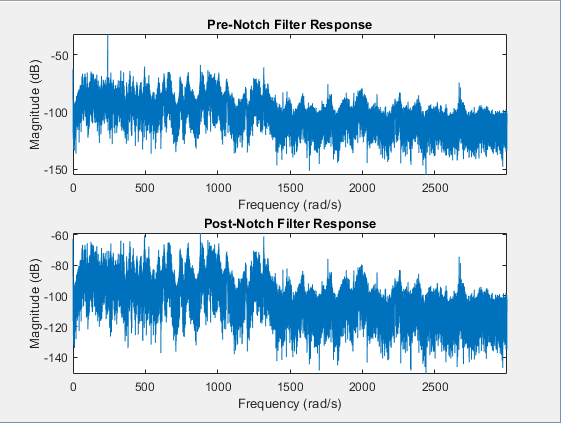
\includegraphics[width = .7\textwidth]{p2p5.png}}
    \end{center}
    \item Document your completion of Part II in the project report:
    \begin{enumerate}
        \item Enter the filter coefficients found in step 1 and plot the corresponding frequency response in units of dB and radians.
        \begin{center}
            The plot for this can be seen under the problem one section.
        \end{center}
        \item Describe the auditory effect of the filter in step 3 and 4. What quality factor did you use?
        \begin{center}
            I decided to use quality factor 35, when I did this the hum in the background completely disappeared and it sounded perfect. I came to the number of 35 by slowly moving up and down the value and listening every time to see how much noise was removed, sometimes it would be too much and some other parts would unintentionally filtered out.
        \end{center}
        \item Describe your observations and plots from step 5.
        \begin{center}
            The plot from 5 was confusing at first because it seems like the overall size of the signal was getting bigger, but rather the axis was re-scaled because the very large spike of noise was removed after the filter and the signal looks much more clean.
        \end{center}
    \end{enumerate}
\end{enumerate}
\newpage
\section*{Part 3: Reconstruction Filter}
\begin{enumerate}
    \item Using the wav2spice program and the step option, convert the output of your digital filter from Part II, step 3 to a PWL file for use in LTSpice as a voltage source. This simulates the conversion from a digital to analog representation, for example using an R-2R ladder
    \item Copy and modify your LTSpice Butterworth filter circuit from part I to create a reconstruction filter. Adjust the voltage source to use the PWL file from step 1. Perform a transient analysis for 60 sec. Again, this will may several minutes, so be patient.
    \begin{center}
        \boxed{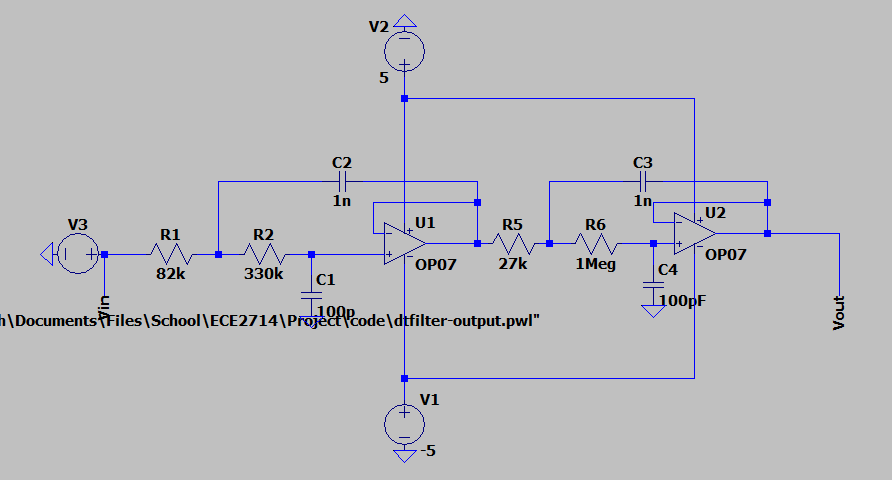
\includegraphics[width = .7\textwidth]{p3p2.png}}
    \end{center}
    \item In LTSpice plot the input and output traces. Zoom in on a few time points so that you can see the details of the signal over a few sampling intervals. Take screenshots and make any observations about the input and output signals.
    \begin{center}
        \boxed{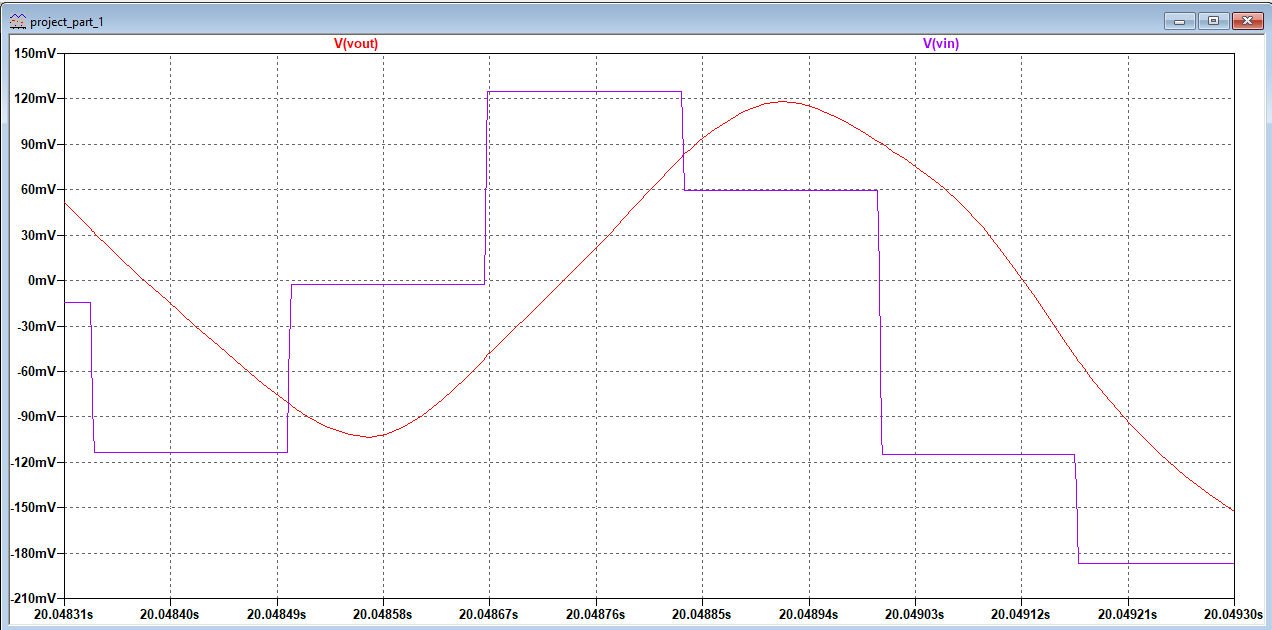
\includegraphics[width = .7\textwidth]{p3p3.png}}
    \end{center}
    \item Document your completion of Part III in the project report:
    \begin{enumerate}
        \item Describe your observations and screenshots from step 4.
        \begin{center}
            The effect the circuit seemed to have is that it smoothened the digital representation of the signal into a signal that can be listened to without artifacts, while also giving it a slight phase shift as a result. This happens similar to how a DC to AC converter works, start with a square wave and use a low pass filter on it to smooth out the edges.
        \end{center}
    \end{enumerate}
\end{enumerate}
\end{document}
